\begin{figure*}
  \centering
  \begin{subfigure}[b]{\textwidth}
    % \begin{noindent}
    \centering
    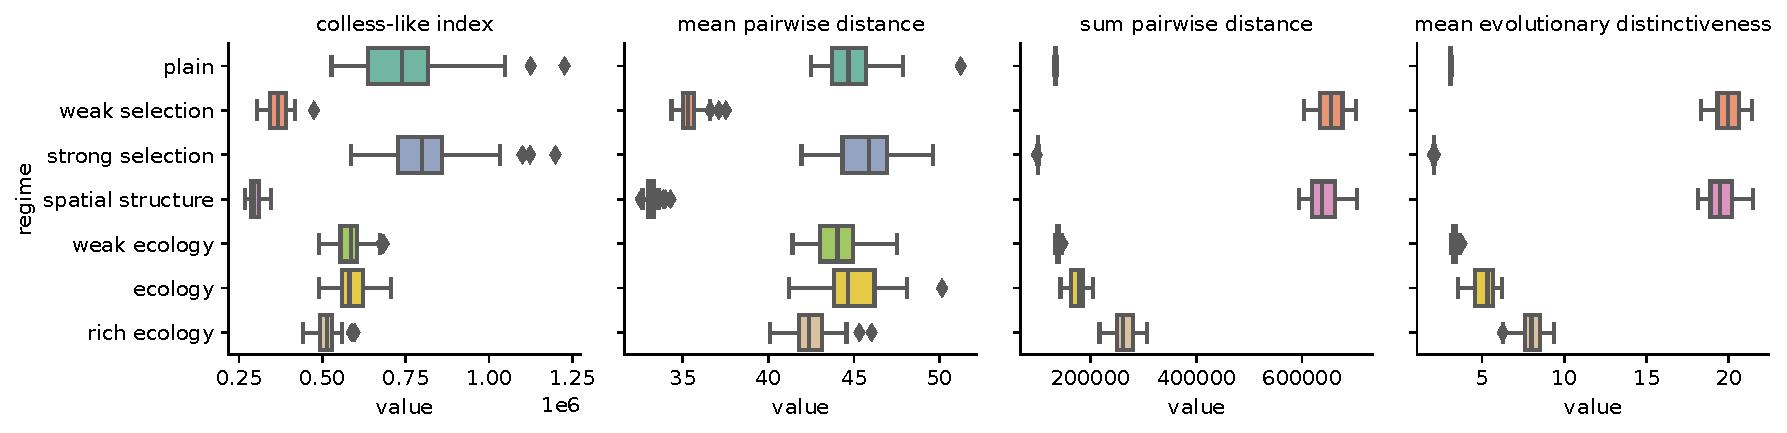
\includegraphics[width=\textwidth]{binder/binder/teeplots/col=phylometric+epoch=0+mut_distn=np.random.standard_normal+viz=boxplot+x=value+y=regime+ext=.pdf}
    % \end{noindent}
    \caption{%
      gaussian mutation distribution at epoch 0 (generation 32,768)}
    \label{fig:perfect-tree-phylometrics-sensitivity-analysis:epoch0}
  \end{subfigure}
  \begin{subfigure}[b]{\textwidth}
    % \begin{noindent}
    \centering
    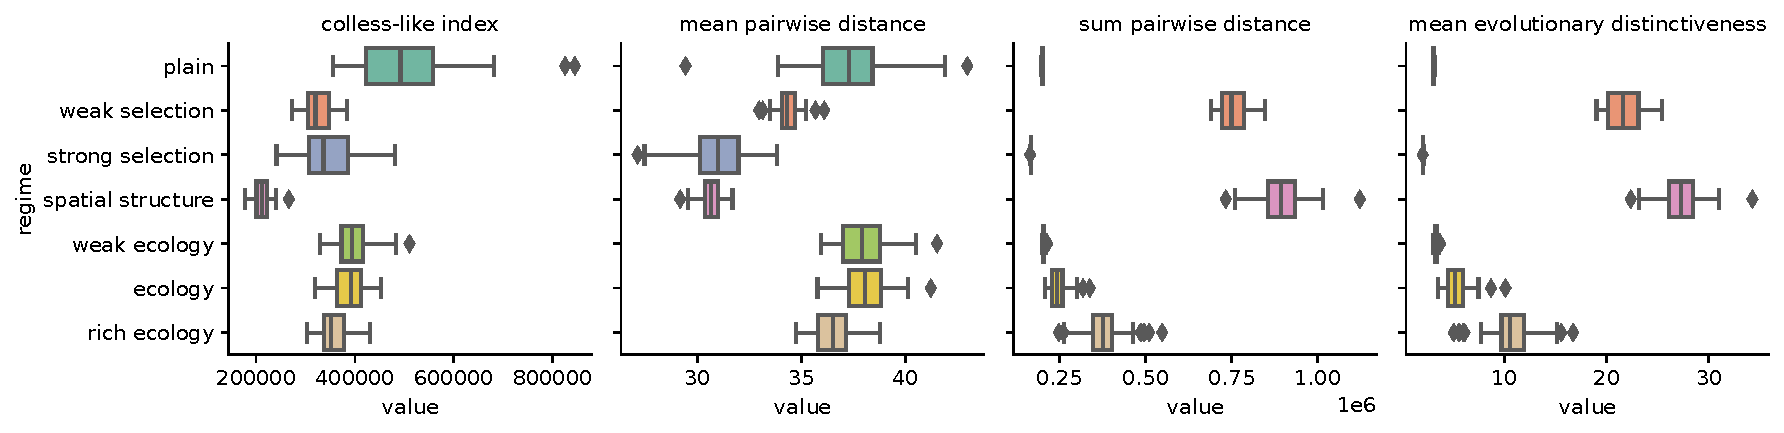
\includegraphics[width=\textwidth]{binder/binder/teeplots/col=phylometric+epoch=2+mut_distn=np.random.standard_normal+viz=boxplot+x=value+y=regime+ext=.pdf}
    % \end{noindent}
    \caption{%
      gaussian mutation distribution at epoch 2 (generation 98,304)}
    \label{fig:perfect-tree-phylometrics-sensitivity-analysis:epoch2}
  \end{subfigure}
  \begin{subfigure}[b]{\textwidth}
    % \begin{noindent}
    \centering
    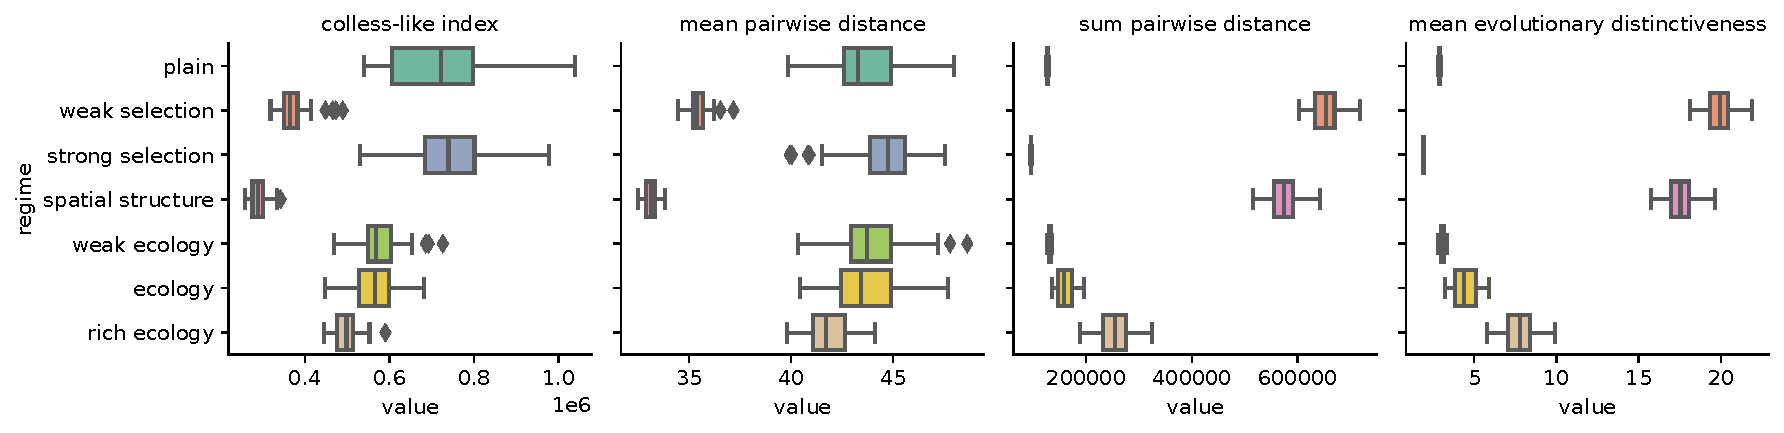
\includegraphics[width=\textwidth]{binder/binder/teeplots/col=phylometric+epoch=0+mut_distn=np.random.exponential+viz=boxplot+x=value+y=regime+ext=.pdf}
    % \end{noindent}
    \caption{%
      exponential mutation distribution at epoch 7 (generation 262,144)}
    \label{fig:perfect-tree-phylometrics-sensitivity-analysis:exponential}
  \end{subfigure}
  % \begin{noindent}
  \caption{
    Distribution of tree phylometrics across surveyed evolutionary regimes for sensitivity analysis conditions.
    Phylometrics were calculated on perfect-fidelity simulation phylogenetic records.
    Sample sizes of $n=50$ replicates define each depicted distribution.
  }
  \label{fig:perfect-tree-phylometrics-sensitivity-analysis}
  % \end{noindent}
\end{figure*}
